\documentclass[12pt,a4paper]{article}
\usepackage{graphicx}
\usepackage[applemac]{inputenc} %% european characters can be used (Mac OS)
% ------------------------------------------------
\usepackage[T1]{fontenc}   %% get hyphenation and accented letters right
\usepackage{mathptmx}      %% use fitting times fonts also in formulas
\pagestyle{empty}                %% no page numbers!
\usepackage[left=35mm, right=35mm, top=15mm, bottom=20mm, noheadfoot]{geometry}

% begin the document
\begin{document}
\thispagestyle{empty}

\title{\textbf{When a Plant Disease Epidemiologist walks on the data science}}
\author{Sith Jaisong \\
Plant Disease Management Group, CESD, IRRI\\ Los Ba\~{n}os, Philippines\\
s.jaisong@irri.org}
\date{} % <--- leave date empty
\maketitle\thispagestyle{empty} %% <-- you need this for the first page
% introduction should have the objective otr the problem or even telling the reader what you wanna say, and 
During I was doing on my research, I found out there are many similarities between plant disease epidemiology and data science. Epidemiologists often deal with more than one factors possibly causing the plant disease. Humidity, temperature, soil pH, soil type, plant varieties, crop density, etc are some examples of variables considering the causes of plant disease development. When the number of variables were added in the study, the dataset will become massive, and require a powerful tool to manage. Data science is emerging to meet the challenge of processing very large dataset (Big Data). It applies the techniques from statistics and computer science extracting the meaning from the data and product the data product (graphs or models, etc.) in order to answer the questions. The process \cite{schutt2013doing} starts with collecting the data that are able to answer the questions or hypothesis. Joining, combining, or wrangling the data are the processes after getting them. In reality data we have may be needed to clean(outlier and missing value removal). Once we have this clean dataset, exploratory data analysis may be applied. Next, Designing the model by using some algorithm k-nearest neighbor (k-NN), linear regression etc. The model selected depend on the type of questions you try to answer. Then, we can interpret, visualize, report or communicate the result. The process of data science is in common with plant disease epidemiology. Epidemiologists often deal with more than one variable possibly causing the plant disease. Plant diseases develop from interaction between plant and its pathogen but also environment (weather) and human activities referring to the agricultural practices. The models are effective features capturing these relationships. They are developed for many uses or objectives. The most common ones are description, understating, prediction, comparison, and communication \cite{madden2007study}. The idea and the process of tackling the problem seem going to the same way. The data science process  

\begin{figure}[h]
%uncomment next line to include a graphic file
\centerline{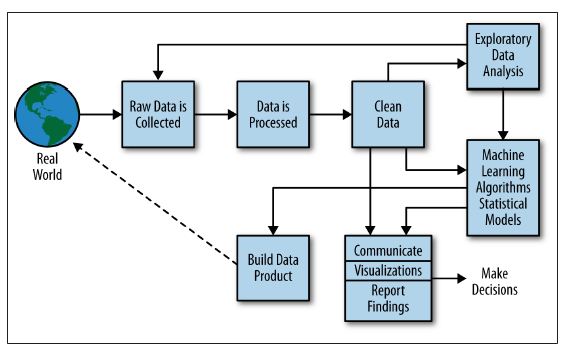
\includegraphics[width=8cm]{Figure2-2}}
%and comment out next line
%\centerline{\framebox[6cm]{\rule{0cm}{3.5cm} figure example}}
\caption{Data science process borrow from \cite{schutt2013doing}}
\label{fig1}
\end{figure}

\bibliography{seminar}
\bibliographystyle{plain}
\end{document}